\section{Introduction}
\subsection{Overview}
Carcassonne is a tile-based board game for two to five players.  The game board
is a medieval landscape built by the players as the game develops. There is a
initial tile on board, and abound 70 other tiles shuffled face down for the
players to draw from.  Each player takes turn to draw a tile and places it
adjacent to tiles that are already on board. The new tile must be placed in
such a way that extends the regions that is at the edge of the tiles it is
adjacent to.  In particular, roads must connect to roads, fields to fields and
cities to cities.  Besides these three types of features, there is another
feature called `cloister'.  After placing a tile, the player can opt to place a
`follower' on a region of the newly-placed tile. The game ends when all the
tiles are placed.  At that time, each follower on board will be scored for
points according to the regions it is occupying.  Traditionally, the human
players have to view the game board and calculate the scores manually. This is
sometimes time consuming, because there may be many regions and followers on
board.  Furthermore, the score rule is based on the concept of regions, which
makes it nearly impossible to calculate the scores in a simple glimpse.  Even
an experienced player may make mistakes due to the potential possibilities of
connectivity of the regions.  Thus, this motivates us to develop a compute
program that can automatically computes the scores given a final game board
setting.  The program can be written as an cell phone application.  The ideal
scenario will be that after playing a game, one can use a cell phone to take a
photo, and the program reports the scores.  Our program is written in Matlab,
but the methodology can be easily implemented and ported to a cell phone using
required programming language.

\begin{figure}[b]
\centering
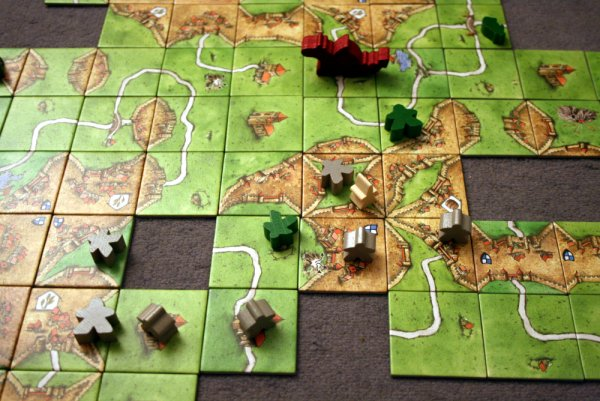
\includegraphics[height=.2\textheight]{board.jpg}
\caption{A part of a game board after several turns (image from
wikipedia).}
\label{fig:board}
\end{figure}

\subsection{Scoring Rules}
Now we introduce the scoring rule after the game finishes.
Note that we deliberately omits the rules when the game is going on,
since we are only focusing on the final game board.
After the game finishes, there will be some incomplete features (regions)
on board. The scoring rules for each feature is as follows:
\begin{itemize}
  \item Road: 1 point per tile.
  \item City: 1 point per tile and 1 point per pennant (a special mark
    that appears in some city features).
  \item Cloister: 1 point itself and 1 point for each surrounding tile.
  \item Field: 3 points for the player who has the most farmers in each
    farm supplying each completed city. This is the most complicated rule,
    since it requires us to explore the field and seek if an adjacent city
    is completed.
\end{itemize}

\subsection{Our Approach}
